\section{CapTap}
\begin{figure}[h]
\centering
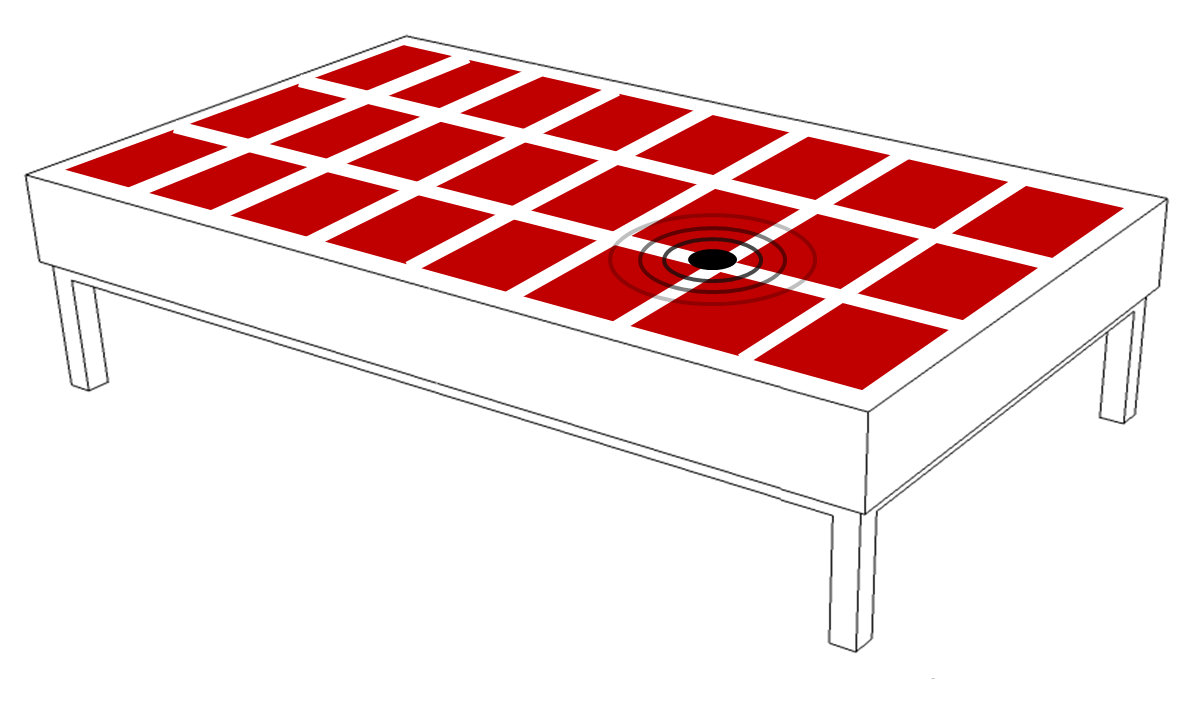
\includegraphics[width=0.7\textwidth]{images/captap_v2}
\caption{CapTap sketch - 24 electrodes placed under table surface}
\label{fig:captap_sketch}
\end{figure}
%Figure 33 CapTap sketch - 24 electrodes placed under table surface
The CapTap is a large area interaction device unobtrusively integrated into a living room table. It is comprised of 24 capacitive sensors and a single sen-sor for knock detection that supports selection events within the demonstration applications [80]. In the domain of free-air gestural interaction there are two prevalent challenges. The physical demands of pro-longed interaction with such systems  is high [81], [82]. Additionally it is difficult to adapt selection events to gestural input. The latter is typically real-ized using time- or position-based gestures [81], [83]. There is no trivial solution to these challenges and any approach has to take into account the specific application scenario covered. Several systems are trying to provide specific GUIs, while others include additional input devices assisting the interaction [84], [85]. CapTap presents an approach to improve the interaction speed of invisible input devices based on capacitive proximity sensors. We have developed a method to unobtrusively detect knocks on a table equipped with a hand tracking system based on capacitive proximity sensors that allows emulating selection events that would typically require an additional time- or movement-based gesture. 
\subsection{Data processing}
\begin{figure}[h]
\centering
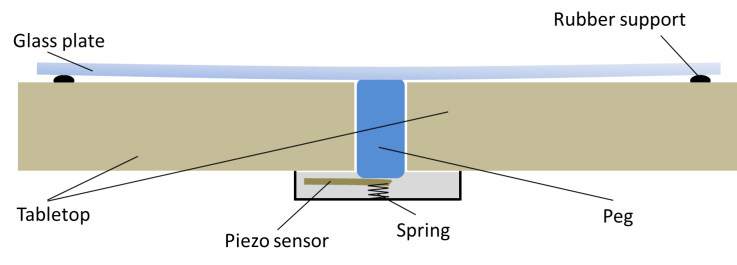
\includegraphics[width=0.7\textwidth]{images/captap_peg}
\caption{Suspended peg knock detection system for CapTap \cite{Braun2013ChairAid}}
\label{fig:captap_peg}
\end{figure}
%Figure 34 Suspended peg knock detection system for CapTap [80]
The hand location of the CapTap is similar to the methods presented for the MagicBox. We add the additional component of knock detection to provide selection events when touching the surface. Figure \ref{fig:captap_sketch} shows a sketch of the knock detection system. The table has a glass plate that is suspended on some rubber supports. In the center of the table we attach a small peg (enlarged in sketch) that creates a connection between the glass plate and a piezo sensor. If the glass plate starts vibrating from a touch we can measure this using the piezo sensor \cite{Braun2013ChairAid}. If a notable vibration is measured we are collecting the next 50 samples, resulting in a window of 250 milliseconds. To distinguish single and double knocks we calculate the weighted average within this window to get a measure for the distribution of sensor values within. If the average is closer to the beginning of the window the resulting event should be a single knock, and a double if the average is closer to the end of the window.
Hand localization and knock detection are working independently and are combined later in the software. It is reasonable to combine this, e.g. to ignore knock events that are occurring without a hand present. They may be indicative of a person doing a strong step close to the table.
\subsection{Evaluation}
\begin{figure}[h]
\centering
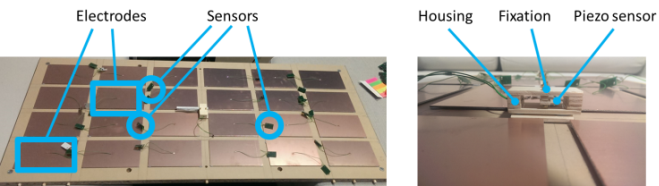
\includegraphics[width=0.7\textwidth]{images/captap_proto}
\caption{Detail views of the prototype system: left - electrode and sensors, right - knock detection box \cite{Braun2013ChairAid}}
\label{fig:captap_proto}
\end{figure}
%Figure 35 Detail views of the prototype system: left - electrode and sensors, right - knock detection box [80]
The CapTap prototype is integrated into a common living room table. Some photos can be seen in Figure \ref{fig:captap_proto}. On the left side we see the 24 electrodes made of non-etched circuit boards. A sensor is attached to each. The knock detection box with fixation, housing and piezo sensor is shown on the right side.
\begin{figure}[h]
\centering
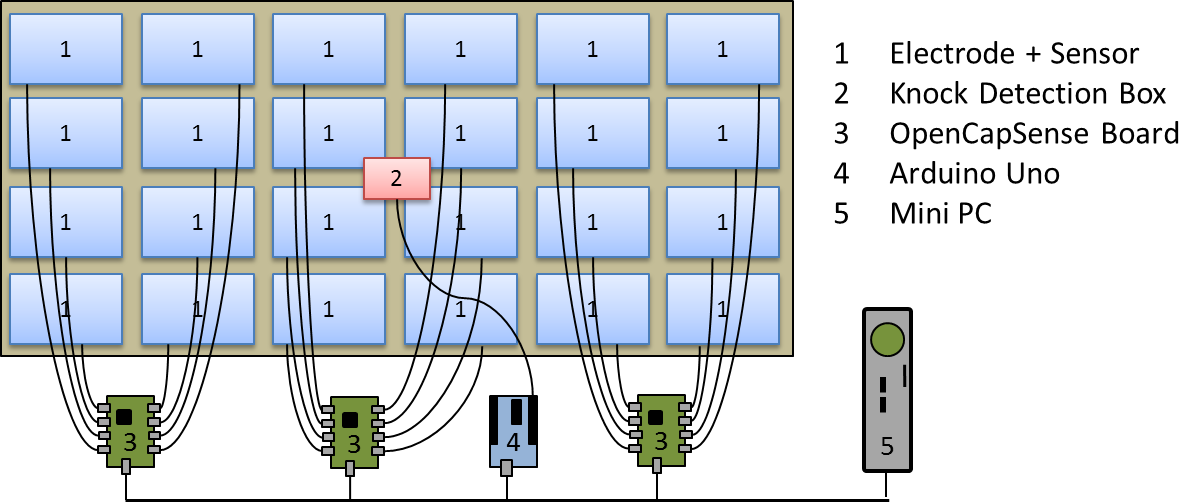
\includegraphics[width=0.7\textwidth]{images/captap_system}
\caption{Abstracted view of CapTap prototype including capacitive sensing electrodes and knock detection sensor \cite{Braun2013ChairAid}}
\label{fig:captap_system}
\end{figure} 
%Figure 36 Abstracted view of CapTap prototype including capacitive sensing electrodes and knock detection sensor [80]
The overall abstracted layout of the prototype is shown in Figure \ref{fig:captap_system}. The capacitive sensors are con-trolled by three OpenCapSense boards; the knock detection is performed on an Arduino Uno microcontroller board. The data fusion is outsourced to a Mini-PC that can be placed in the table.
Various evaluations have been performed with the CapTap. We have benchmarked the hand localization against the Leap Motion, concluding that the algorithm works reasonably precise in most parts of the interaction area. The next study was a quantitative study of the percentage of correctly recognized knocks, resulting in considerable misattribution of single and double knocks, due to strongly varying knocking styles. However, the presence of any knock was detected with a precision of about $90\%$ \cite{Braun2013ChairAid}. Our main evaluation of the system was concerned with the influence of our knock detection on the overall interaction speed of the system. The results concluded that merely adding the knock detection is not enough but that additionally the interfaces have to be adapted towards capacitive systems \cite{Braun2013ChairAid}.
